\hypertarget{results}{%
\section{Results}\label{results}}

\hypertarget{the-ground-state-flux-sector}{%
\subsection{The Ground State Flux
Sector}\label{the-ground-state-flux-sector}}

Here I will discuss the numerical evidence that our guess for the ground
state flux sector is correct, it relies on three key numerical
observations arguments:

First we fully eumerate the flux sectors of \textasciitilde25,000
periodic systems with a disordered unit cell of up to 16 plaquettes
(\(2^{16-1}\) sectors). Going to larger system sizes in impractical
because of the exponential sclaling. However, as discussed earlier,
finite size effects play a large role for small systems
\autocite{kitaevAnyonsExactlySolved2006}. To get around this we look at
periodic systems with amorphous unit cells. This reduces the finite size
effects but we can use Bloch's theorem to diagonalise periodic systems
with only a linear penalty in system area.

Looking at periodic systems comes at the expense of removing
longer-range disorder from our lattices so we bolster this by comparing
the behaviour of periodic lattice with amorphous to unit cells to fully
amorphous lattice as we scale the size of the unit cell. We show that
the energetic effect of introducing perodicity scales away as we go to
larger system sizes.

From these two observations we argue that the results for small periodic
systems generalise to large amorphous systems. We perform this analysis
for both the isotropic point (\(J^\alpha = 1\)), as well as in the toric
code phase (\(J^x = J^y = 0.25, J^z = 1\)).

In the isotropic case (\(J^\alpha = 1\)), our conjecture correctly
predicted the ground state flux sector for all of the lattices we
tested.

For the toric code phase (\(J^x, J^y = 0.25, J^z = 1\)) all but around
(\(\sim 0.5 \%\)) lattices had ground states conforming to our
conjecture. In these cases, the energy difference between the true
ground state and our prediction was on the order of \(10^{-6} J\). It is
unclear whether this is a finite size effect or something else.

\hypertarget{spontaneous-chiral-symmetry-breaking}{%
\subsection{Spontaneous Chiral Symmetry
Breaking}\label{spontaneous-chiral-symmetry-breaking}}

The spin Kitaev Hamiltonian is real and therefore has time reveral
symmetry. However, the flux \(\phi_p\) through any plaquette with an odd
number of sides has imaginary eigenvalues \(\pm i\). Further we have
shown that the ground state sector induces a relatively regular pattern
for the imaginary fluxes with only a global two-fold degeneracy.

Thus, states with a fixed flux sector spontaneously break time reversal
symmetry. This was first described by Yao and Kivelson~for a translation
invariant Kitaev model with odd sided plaquettes \autocite{Yao2011}.

Thus we have flux sectors that come in degenerate pairs, where time
reversal is equivalent to inverting the flux through every odd
plaquette, a general feature for lattices with odd
plaquettes~\autocite{yaoExactChiralSpin2007,Peri2020}. This
spontaneously broken symmetry avoids the need to explicitly break TRS
with a magnetic field term as is done in the original honeycomb model.

\hypertarget{ground-state-phase-diagram}{%
\subsection{Ground State Phase
Diagram}\label{ground-state-phase-diagram}}

As previously discusssed, the standard Honeycomb model has a Abelian,
gapped phase in the anisotropic region and is gapless in the isotropic
region. The introduction of a magnetic field breaks the chiral symmetry,
leading to the isotropic region becoming a gapped, non-Abelian phase.

Similar to the Kitaev Honeycomb model with a magnetic field, we find
that this model is only gapless along critical lines, see
\textasciitilde{}\ref{fig:phase_diagram} (Left). Interestingly, the gap
closing exists in only one of the four topological sectors, though this
is certainly a finite size effect as the sectors must become degenerate
in the thermodynamic limit.

In the honeycomb model, the phase boundaries are located on the straight
line \(|J^x| = |J^y| + |J^x|\) and permutations of \(x,y,z\), shown as
dotted line on \textasciitilde{}\ref{fig:phase_diagram} (Right). We find
that on the amorphous lattice these boundaries exhibit an inward
curvature, similar to honeycomb Kitaev models with flux
\autocite{Nasu_Thermal_2015} or bond \autocite{knolle_dynamics_2016}
disorder.

\begin{figure}
\hypertarget{fig:phase_diagram}{%
\centering
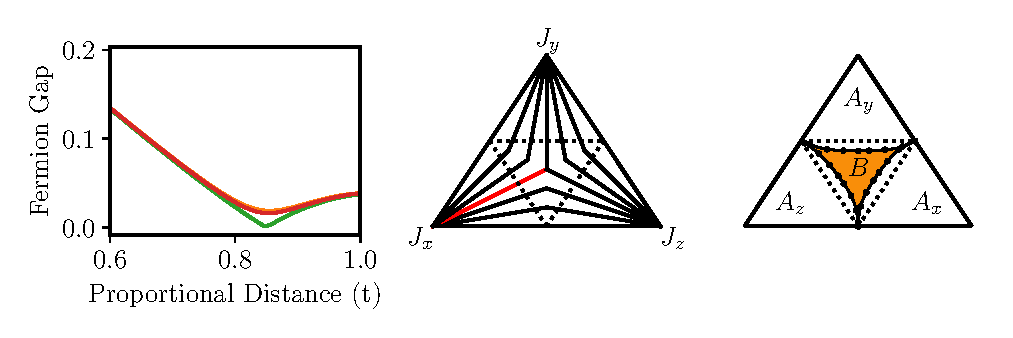
\includegraphics[width=1\textwidth,height=\textheight]{figure_code/amk_chapter/results/phase_diagram/phase_diagram.pdf}
\caption{(Center) We choose an energy scale for the Hamiltonian by
setting \(J_x + J_y + J_z = 1\). This intersects a plane with the unit
cube spanned by \(J_\alpha \in [0,1]\), giving a triangle with corners
\((1,0,0), (0,1,0), (0,0,1)\). To compute critical lines efficiently in
this space we evaluate the order parameter of interest along rays
shooting from the corners. The ray highlighted in red defines the values
of J used for the left figure. (Left) The fermion gap as a function of J
for an amorphous system with 20 plaquettes, where the x axis is the
position on the red line in the central figure from 0 to 1. For finite
size systems the four topological sectors are not degenerate and only
one of them has a true gap closing. (Right) The Abelian \(A_\alpha\)
phases of the model and the non-Abelian B phase separated by critical
lines where the fermion gap closes. Later we will show that the chern
number \(\nu\) changes from \(0\) t0 \(\pm 1\) from the A phases to the
B phase.}\label{fig:phase_diagram}
}
\end{figure}

\hypertarget{is-it-abelian-or-non-abelian}{%
\subsubsection{Is it Abelian or
non-Abelian?}\label{is-it-abelian-or-non-abelian}}

The two phases of the amorphous model are clearly gapped, though see
later for a finite size scaling check on this.

The next question is: do these phases support Abelian or non-Abelian
statistics? To answer that we turn to Chern numbers and markers. As
discussed earlier the Chern number is a quantity intimately linked to
both the topological properties and the anyonic statistics of a model.
The Abelian/non-Abelian character of a model is linked to its Chern
number \textbf{citation}. However the Chern number is only defined for
the translation invariant case.

A family of generalisations to amorphous systems exist
\autocite{mitchellAmorphousTopologicalInsulators2018} called local
topological markers. We use the crosshair marker
\textcite{peru_preprint} here to assess the Abelian/non-Abelian
character of the phases.

Like the honeycomb model, the amorphous model retains an Abelian gapped
phase in the anisotropic region with \(\nu=0\). This phase is the
amorphous analogue of the abelian toric-code quantum spin liquid
\autocite{kitaev_fault-tolerant_2003}.

The isotropic region has \(\nu=\pm1\) so is a non-Abelian chiral spin
liquid (CSL) similar to that of the Yao-Kivelson model
\autocite{yaoExactChiralSpin2007}. Hereafter we focus our attention on
this phase.

\begin{figure}
\hypertarget{fig:phase_diagram_chern}{%
\centering
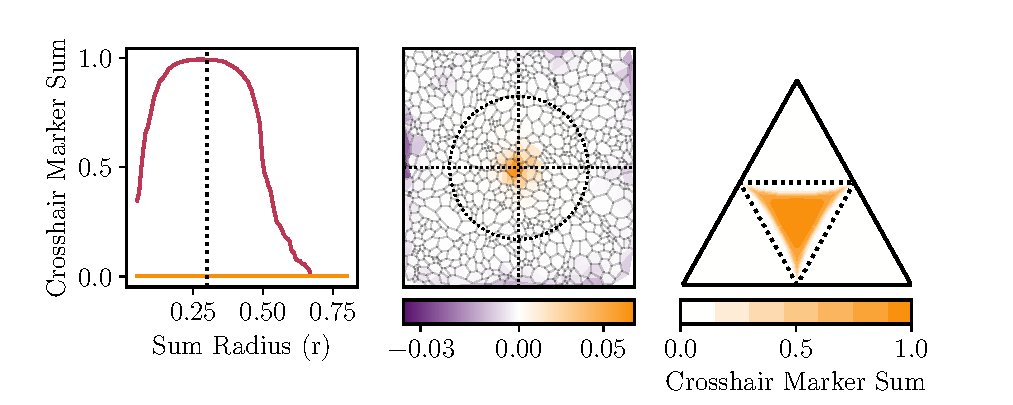
\includegraphics[width=1\textwidth,height=\textheight]{figure_code/amk_chapter/results/phase_diagram_chern/phase_diagram_chern.pdf}
\caption{(Center) The crosshair marker \textcite{peru_preprint}, a local
topological marker, evaluated on the Amorphous Kitaev Model. The marker
is defined around a point, denoted by the dotted crosshair. Information
about the local topological properties of the system are encoded within
a region around that point. (Left) Summing these contributions up to
some finite radius (dotted line here, dotted circle in the center) gives
a generalised version of the Chern number for the system which becomes
quantised in the thermodynamic limit. The radius must be chosen large
enough to capture information about the local properties of the lattice
while not so large as to include contributions from the edge states. The
isotropic regime \(J_\alpha = 1\) in red has \(\nu = \pm 1\) implying it
supports excitations with non-Abelian statistics, while the anisotropic
regime in orange has \(\nu = \pm 0\) implying it has Abelian statistics.
(Right) Extending this analysis to the whole \(J_\alpha\) phase diagram
with fixed \(r = 0.3\) nicely confirms that the isotropic phase is
non-Abelian.}\label{fig:phase_diagram_chern}
}
\end{figure}

\hypertarget{chern-number-and-edge-modes}{%
\subsubsection{Chern Number and Edge
Modes}\label{chern-number-and-edge-modes}}

The QSLs separated by these lines are distinguished by a real-space
analogue of the Chern number
\autocite{bianco_mapping_2011,Hastings_Almost_2010}. A similar
topological number was discussed by Kitaev on the honeycomb lattice
\autocite{kitaevAnyonsExactlySolved2006} that we shall use here with a
slight modification
\autocite{peru_preprint,mitchellAmorphousTopologicalInsulators2018}. For
a choice of flux sector, we calculate the projector \(P\) onto the
negative energy eigenstates of the matrix \(iA\) defined in
eqn.~\protect\hyperlink{eqn:majorana_hamiltonian}{{[}eqn:majorana\_hamiltonian{]}}.
The local Chern number around a point \(\textbf{R}\) in the bulk is
given by \[\begin{aligned}
    \nu (\textbf{R}) = 4\pi \Im \mathrm{Tr}_{\mathrm{Bulk}} 
    \left ( 
    P\theta_{R_x} P \theta_{R_y} P
    \right ),\end{aligned}\] where \(\theta_{R_x}\) is a step function
in the \(x\)-direction, with the step located at \(x = R_x\),
\(\theta_{R_y}\) is defined analogously. The trace is taken over a
region around \(\textbf{R}\) in the bulk of the material, where care
must be taken not to include any points close to the edges. Provided
that the point \(\textbf{R}\) is sufficiently far from the edges, this
quantity will be very close to quantised to the Chern number.

The local Chern marker distinguishes between an Abelian phase (A) with
\(\nu = 0\), and a non-Abelian (B) phase characterized by
\(\nu = \pm 1\). The (A) phase is equivalent to the toric code on an
amorphous system \autocite{kitaev_fault-tolerant_2003}.

Since the (A) phase displays the "topological" degeneracy described
above, I think that "topologically trivial" is not a good term to
describe it. Another thing that I think it should be considered here.
The abelian phase is expected to have 2x4 degeneracy, where the factor
of 2 comes from time-reversal. On the other hand, the non-Abelian phase
should display 2x3 degeneracy, as discussed by
\autocite{yaoExactChiralSpin2007}. Did you get any evidence of this?

By contrast, the (B) phase is a \emph{chiral spin liquid}, the magnetic
analogue of the fractional quantum Hall state. Topologically protected
edge modes are predicted to occur in these states on periodic boundary
conditions following the bulk-boundary correspondence
\autocite{qi_general_2006}. The probability density of one such edge
mode is given in \protect\hyperlink{fig:edge_modes}{1} (a), where it is
shown to be exponentially localised to the boundary of the system. The
localization of these modes can be quantified by their inverse
participation ratio (IPR),
\[\mathrm{IPR} = \int d^2r|\psi(\mathbf{r})|^4  \propto L^{-\tau},\]
where \(L\sim\sqrt{N}\) is the characteristic linear dimension of the
amorphous lattices and \(\tau\) dimensional scaling exponent of IPR.

Finally, the CSL density of states in open boundary conditions indicates
the low-energy modes within the gap of Majorana bands in
\protect\hyperlink{fig:edge_modes}{1} (b).

The phase diagram of the amorphous model in
\protect\hyperlink{fig:example_lattice}{{[}fig:example\_lattice{]}}(c)
displays a reduced parameter space for the non-Abelian phase when
compared to the honeycomb model. Interestingly, similar inward
deformations of the critical lines were found on the Kitaev honeycomb
model subject to disorder by proliferating flux vortices
\autocite{Nasu_Thermal_2015} or exchange disorder
\autocite{knolle_dynamics_2016}.

\begin{figure}
\hypertarget{fig:figure_2_bashed}{%
\centering
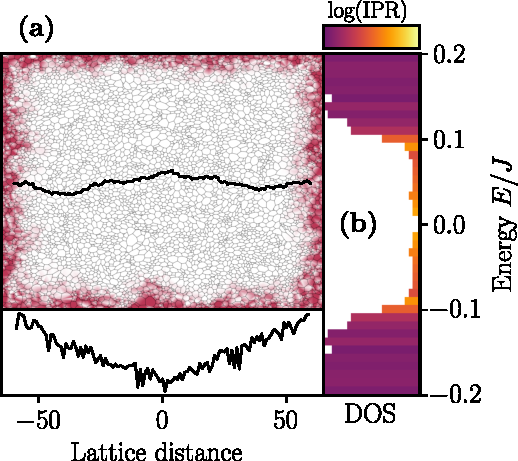
\includegraphics[width=0.57\textwidth,height=\textheight]{figure_code/amk_paper/figure_2_bashed.pdf}
\caption{}\label{fig:figure_2_bashed}
}
\end{figure}

\hypertarget{anderson-transition-to-a-thermal-metal}{%
\subsection{Anderson Transition to a Thermal
Metal}\label{anderson-transition-to-a-thermal-metal}}

\begin{figure}
\hypertarget{fig:fermion_gap_vs_L}{%
\centering
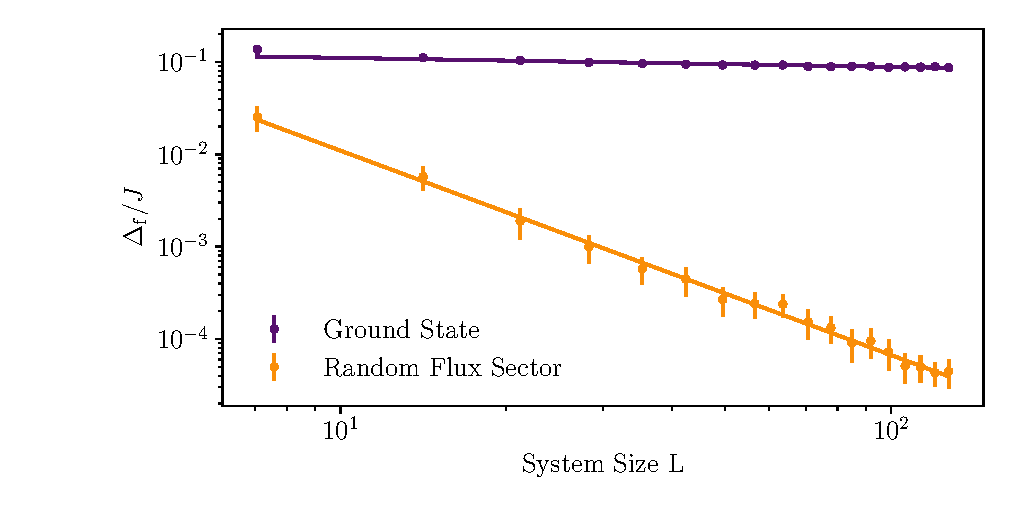
\includegraphics[width=1.14\textwidth,height=\textheight]{figure_code/amk_chapter/results/fermion_gap_vs_L/fermion_gap_vs_L.pdf}
\caption{Within a flux sector, the fermion gap \(\Delta_f\) measures the
energy between the fermionic ground state and the first excited state.
This graph shows the fermion gap as a function of system size for the
ground state flux sector and for a configuration of random fluxes. We
see that the disorder induced by an putting the Kitaev model on an
amorphous lattice does not close the gap in the ground state. The gap
closes in the flux disordered limit is good evidence that the system
transitions to a gapless thermal metal state at high temperature. Each
point shows an average over 100 lattice realisations. System size \(L\)
is defined \(\sqrt{N}\) where N is the number of plaquettes in the
system. Error bars shown are \(3\) times the standard error of the mean.
The lines shown are fits of \(\tfrac{\Delta_f}{J} = aL ^ b\) with fit
parameters: Ground State: \(a = 0.138 \pm 0.002, b = -0.0972 \pm 0.004\)
Random Flux Sector:
\(a = 1.8 \pm 0.2, b = -2.21 \pm 0.03\)}\label{fig:fermion_gap_vs_L}
}
\end{figure}

a thermal-induced Anderson transition to a thermal metal phase
\autocite{selfThermallyInducedMetallic2019}.

An Ising non-Abelian anyon is formed by Majorana zero-modes bound to a
topological defect \autocite{Beenakker2013}. Interactions between anyons
are modeled by pairwise projectors whose strength absolute value decays
exponentially with the separation between the particles, and whose sign
oscillates in analogy to RKKY exchanges
\autocite{Laumann2012,Lahtinen_2011,lahtinenTopologicalLiquidNucleation2012}.
Disorder can induce a finite density of anyons whose hybridization lead
to a macroscopically degenerate state known as \emph{thermal metal}
\autocite{Laumann2012}. One instance of this phase can be settled on the
Kitaev CSL. In this case, the topological defects correspond to the
\(W_p \neq +1\) fluxes, which naturally emerge from thermal fluctuations
at nonzero temperature \autocite{selfThermallyInducedMetallic2019}.

We demonstrated that the amorphous CSL undergoes the same form of
Anderson transition by studying its properties as a function of
disorder. Unfortunately, we could not perform a complete study of its
properties as a function of the temperature as it was not feasible to
evaluate an ever-present boundary condition dependent factor
\autocite{pedrocchiPhysicalSolutionsKitaev2011,Zschocke_Physical_states2015}
for random networks. Instead, we evaluated the fermionic density of
states (DOS) and the IPR as a function of the vortex density \(\rho\) as
a proxy for temperature. This approximation is exact in the limits
\(T = 0\) (corresponding to \(\rho = 0\)) and \(T \to \infty\)
(corresponding to \(\rho = 0.5\)). At intermediate temperatures the
method neglects to include the influence of defect-defect correlations.

However, such an approximation is enough to show the onset of low-energy
excitations for \(\rho \sim 10^{-2}-10^{-1}\), as displayed on the top
graphic of
\protect\hyperlink{fig:DOS_Oscillations}{{[}fig:DOS\_Oscillations{]}}(a).
We characterized these gapless excitations using the dimensional scaling
exponential \(\tau\) of the IPR on the bottom graphic of the same
figure. At small \(\rho\), the states populating the gap possess
\(\tau\approx0\), indicating that they are localised states pinned to
the defects, and the system remains insulating. At large \(\rho\), the
in-gap states merge with the bulk band and become extensive, closing the
gap, and the system transitions to a metallic phase.

The thermal metal DOS displays a logarithmic divergence at zero energy
and characteristic oscillations at small energies.
\autocite{bocquet_disordered_2000,selfThermallyInducedMetallic2019}.
These features were indeed observed by the averaged density of states in
the \(\rho = 0.5\) case shown in
\protect\hyperlink{fig:DOS_Oscillations}{{[}fig:DOS\_Oscillations{]}}(b)
for amorphous lattice. We emphasize that the CSL studied here emerges
without an applied magnetic field as opposed to the CSL on the honeycomb
lattice studied in Ref. \autocite{selfThermallyInducedMetallic2019} I
have the impression that
\protect\hyperlink{fig:DOS_Oscillations}{{[}fig:DOS\_Oscillations{]}}(b)
on the top is very similar to Fig. 3 of
\autocite{selfThermallyInducedMetallic2019}. Maybe a more instructive
figure would be the DOS of the amorphous toric code at the infinite
temperature limit. In this case, the lack of non-Abelian anyons would be
reflected by a gap on the DOS, which would contrast nicely to the
thermal metal phase

\begin{figure}
\hypertarget{fig:figure_3_bashed}{%
\centering
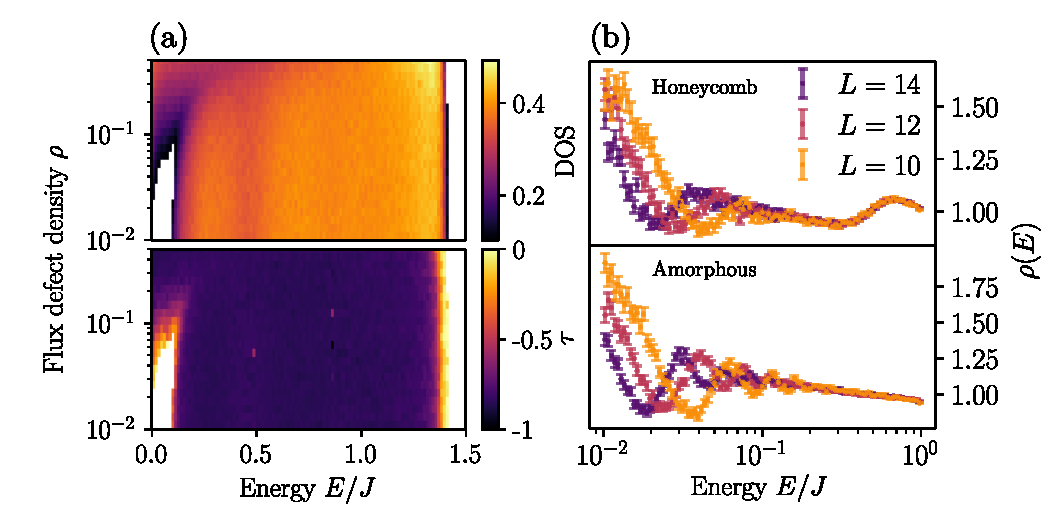
\includegraphics[width=1\textwidth,height=\textheight]{figure_code/amk_paper/figure_3_bashed.pdf}
\caption{}\label{fig:figure_3_bashed}
}
\end{figure}

\hypertarget{conclusion}{%
\section{Conclusion}\label{conclusion}}

We have studied an extension of the Kitaev honeycomb model to amorphous
lattices with coordination number \(z= 3\). We found that it is able to
support two quantum spin liquid phases that can be distinguished using a
real-space generalisation of the Chern number. The presence of odd-sided
plaquettes on these lattices let to a spontaneous breaking of time
reversal symmetry, leading to the emergence of a chiral spin liquid
phase. Furthermore we found evidence that the amorphous system undergoes
an Anderson transition to a thermal metal phase, driven by the
proliferation of vortices with increasing temperature.

\hypertarget{discussion}{%
\section{Discussion}\label{discussion}}

\hypertarget{failure-of-the-ground-state-conjecture}{%
\subsection{Failure of the ground state
conjecture}\label{failure-of-the-ground-state-conjecture}}

We did find a small number of lattices for the ground state conjecture
did not correctly predict the true ground state flux sector. I see two
possibilities for what could cause this.

Firstly it could be a a finite size effect that is somehow amplfied by
certain rare lattice configurations. It would be interesting to try to
elucidate what lattice features are present when the ground state
conjecture fails.

Alternatively, it might be telling that the ground state conjecture
failed in the toric code phase where the couplings are anisotropic.
Clearly the colouring does not matter much in the isotropic phase.
However an avenue that I did not explore was whether the particular
choice of colouring for a lattice affects the physical properties in the
toris code phase. It is possible that some property of the particular
colouring chosen is what leads to failure of the ground state conjecture
here.

\hypertarget{full-monte-carlo}{%
\subsection{Full Monte Carlo}\label{full-monte-carlo}}

\hypertarget{outlook}{%
\section{Outlook}\label{outlook}}

\hypertarget{experimental-realisations-and-signatures}{%
\subsection{Experimental Realisations and
Signatures}\label{experimental-realisations-and-signatures}}

The next step is to search for an experimental realisation in amorphous
Kitaev materials, which can be created from crystalline ones using
several methods \autocite{Weaire1976,Petrakovski1981,Kaneyoshi2018}.

Following the evidence for an induced chiral spin liquid phase in
crystalline Kitaev materials
\autocite{Kasahara2018,Yokoi2021,Yamashita2020,Bruin2022}, it would be
interesting to investigate if a similar state is produced on its
amorphous counterpart.

Probably one way to make this theory experimentally relevant is to do
experiments on amorphous phases of Kitaev materials. These phases can be
obtained by liquifying the material and cooling it fast. Apparently,
most of crystalline magnets can be transformed into amorphous ones
through this process.

Besides the usual half-quantized signature on thermal Hall effect
\autocite{Kasahara2018,Yokoi2021,Yamashita2020,Bruin2022}, such a CSL
could be also characterized using local probes such as spin-polarized
scanning-tunneling microscopy
\autocite{Feldmeier2020,Konig2020,Udagawa2021}. The same probes would
also be useful to manipulate non-Abelian anyons \autocite{Pereira2020},
thereby implementing elementary operations for topological quantum
computation. Finally, the thermal metal phase can be diagnosed using
bulk heat transport measurements \autocite{Beenakker2013}.

\hypertarget{generalisations}{%
\subsection{Generalisations}\label{generalisations}}

This work could be generalized in several ways.

Introduction of symmetry allowed perturbations on the model
\autocite{Rau2014,Chaloupka2010,Chaloupka2013,Chaloupka2015,Winter2016}.

Generalizations to higher-spin models in random networks with different
coordination numbers
\autocite{Baskaran2008,Yao2009,Nussinov2009,Yao2011,Chua2011,Natori2020,Chulliparambil2020,Chulliparambil2021,Seifert2020,WangHaoranPRB2021,Wu2009}
